\documentclass{book} \usepackage{exsheets} \usepackage{xeCJK}
\usepackage{amsmath,amsfonts,amsthm,amssymb} \usepackage{bm}
\usepackage{hyperref} \usepackage{yhmath} \usepackage{caption}
\usepackage{pstricks-add} \usepackage{framed,mdframed}
\usepackage{graphicx,color} \usepackage{mathrsfs,xcolor}
\usepackage[all]{xy} \usepackage{fancybox}
\setcounter{MaxMatrixCols}{20}
\setCJKmainfont[BoldFont=SimHei]{SimSun} \SetupExSheets{
  counter-format = ch.se.qu , counter-within = section, solution/print
  = true }
\begin{document}
\chapter{正交射影和最小二乘法}
\section{内积和转置}
\begin{question}
  \begin{itemize}
  \item 任给两个正数$x$和$y$,作向量$b=(\sqrt{x},\sqrt{y})$,并取
    $a=(\sqrt{y},\sqrt{x})$.利用Schwarz不等式比较$x$和$y$的算术平均值
    与它们的几何平均值的大小.
\item 设我们有一个从原点到点$x$的向量,再加上一个由$x$出发长度为$||y||$
  的向量$x+y$,三角形的第三边直接由原点到$x+y$连结而成,三角不等式断言,
  这个距离不大于前两者之和:
$$
||x+y||\leq ||x||+||y||
$$
两边平方之后进行化简,由此推出Schwarz不等式.
  \end{itemize}
\end{question}
\begin{solution}
  \begin{itemize}
  \item 由Schwarz不等式,
$$
b\cdot a=\sqrt{x}\sqrt{y}+\sqrt{y}\sqrt{x}\leq
\sqrt{x+y}\sqrt{x+y}=||b||\cdot ||a||,
$$
所以
$$
\sqrt{xy}\leq \frac{x+y}{2}.
$$
\item $||x+y||^2=x^2+y^2+2x\cdot y\leq
  (||x||+||y||)^2=x^2+y^2+2||x||\cdot ||y||$.所以
$x\cdot y\leq ||x||\cdot ||y||$.
  \end{itemize}
\end{solution}
\begin{question}
  对图3.3中的三角形$Obp$,使用(5)式来求$bp$的长度,从而验证勾股定理.
\end{question}
\begin{solution}
  略.
\end{solution}
\begin{question}
  在连接原点与$a=(1,1,1)$的射线上求一点$p$,使之距点$b=(2,4,4)$最近.同
  样地.在过$b$的射线上求距$a$最近的点.
\end{question}
\begin{solution}
  \begin{itemize}
  \item
    $p=\frac{ab^T}{aa^{T}}a=(\frac{10}{3},\frac{10}{3},\frac{10}{3})$.
\item $\frac{ab^T}{bb^T}b=(\frac{5}{9},\frac{10}{9},\frac{10}{9})$.
  \end{itemize}
\end{solution}
\begin{question}
  解释一下为什么当$a,b$同时在一条过原点的直线上,且仅在这种情况
  下,Schwarz不等式成为等式.如果它们分别位于原点的两边又如何?
\end{question}
\begin{solution}
  略.
\end{solution}
\begin{question}
  在$n$维空间中,向量$(1,1,\cdots,1)$与各个坐标轴的夹角是什么?
\end{question}
\begin{solution}
  $\cos\theta=\frac{1}{\sqrt{n}}$.所以$\theta=\arccos \frac{1}{\sqrt{n}}$.
\end{solution}
\begin{question}
  如果把$a$和$b$事先化为单位向量的话,Schwarz不等式还有另一个证明:
$$
|a^Tb|=\left| \sum a_ib_i   \right|\leq\sum |a_ib_i|\leq \sum \frac{a_i^2+b_i^2}{2}=\frac{1}{2}+\frac{1}{2}=1=|a||b|
$$
请验证中间的步骤.
\end{question}
\begin{solution}
  略.
\end{solution}
\begin{question}
通过把$AA^{-1}=I$转置,我们发现逆矩阵的转置等于转置的逆矩
阵:$(A^{-1})^T=(A^T)^{-1}$.证明:若$A$对称,则$A^{-1}$也是对称的.
\end{question}
\begin{solution}
  当$A$是对称矩阵时,$(A^{-1})^T=(A^T)^{-1}=A^{-1}$.所以$A^{-1}$也是对
  称矩阵.
\end{solution}
\begin{question}
  构造$2\times 2$对称矩阵$A$和$B$,使得它们的乘积不是对称的.注意若$A$和
  $B$可交换,则乘积仍是对称的.$(AB)^T=B^TA^T=BA=AB$.
\end{question}
\begin{solution}
$$
\begin{pmatrix}
  1&2\\
  2&1
\end{pmatrix}
\begin{pmatrix}
  1&-1\\
  -1&2
\end{pmatrix}=
\begin{pmatrix}
  -1&3\\
  1&0
\end{pmatrix}.
$$
\end{solution}
\begin{question}
  若$A$的秩为$r$,则矩阵$A^T$(行秩=列秩),$A^TA$(由3F)和$AA^T$(3F应用于
  $A^T$)的秩也都是$r$.给出一个例子来说明即使当$A^TA$是可逆的,$AA^T$完
  全可能不是可逆的.
\end{question}
\begin{solution}
反例:令$A=
\begin{pmatrix}
  1&2\\
  -1&-2\\
  1&-1
\end{pmatrix}.
$则
$$
A^TA=
\begin{pmatrix}
  1&-1&1\\
  2&-2&-1
\end{pmatrix}
\begin{pmatrix}
  1&2\\
-1&-2\\
1&-1
\end{pmatrix}=
\begin{pmatrix}
  3&3\\
  3&9
\end{pmatrix},
$$
该矩阵可逆.
$$
AA^T=
\begin{pmatrix}
  1&2\\
  -1&-2\\
  1&-1
\end{pmatrix}
\begin{pmatrix}
  1&-1&1\\
  2&-2&-1
\end{pmatrix}=
\begin{pmatrix}
  5&-5&-1\\
  -5&5&1\\
  -1&1&2
\end{pmatrix}.
$$
该矩阵不可逆.事实上,只要矩阵$A$的行数大于列数,且矩阵$A$是列满秩矩阵,构
造出来的都是反例.
\end{solution}
\begin{question}
  甲烷分子排列成如下形式:碳原子位于一个正四面体的中心,而四个氢原子位
  于顶点上.如果顶点位于$(0,0,0)$,$(1,1,0)$,$(1,0,1)$,$(0,1,1)$——注意所
  有的$6$条棱的棱长都等于$\sqrt{2}$,所以四面体是正四面体.那么,过中心
  $(\frac{1}{2},\frac{1}{2},\frac{1}{2})$和顶点的连线之间的夹角是多少?
\end{question}
\begin{solution}
  略.
\end{solution}
\section{到子空间上的射影和最小二乘逼近}
\begin{question}
  假设我们在四个不同的场合观察一个病人的重量,其结果
  是$b_1=150,b_2=153,b_3=150,b_4=151$,问在最小二乘意义下,我们可认定的体
  重最佳值是多少?
\end{question}
\begin{solution}
  即求方程组
$$
\begin{cases}
  x=150\\
  x=153\\
  x=150\\
  x=151
\end{cases}
$$
的最小二乘解.即求方程组
$$
\begin{pmatrix}
  1\\
  1\\
  1\\
  1\\
\end{pmatrix}x=
\begin{pmatrix}
  150\\
  153\\
  150\\
  151
\end{pmatrix}
$$
的最小二乘解.该方程组的最小二乘解为
$$
\overline{x}=\frac{150\cdot 1+153\cdot 1+150\cdot 1+151\cdot
  1}{1^2+1^2+1^2+1^2}=150.5.
$$
\end{solution}
\begin{question}
  对$3x=10,4x=5$求最小二乘解.
\end{question}
\begin{solution}
  即求线性方程组
$$
\begin{pmatrix}
  3\\
  4
\end{pmatrix}x=
\begin{pmatrix}
  10\\
  5
\end{pmatrix}
$$
的最小二乘解.为
$$
\overline{x}=\frac{10\times 3+5\times 4}{3^2+4^2}=2.
$$
\end{solution}
\begin{question}
  使用正规方程,求下列不相容方程组在最小二乘意义下的最佳解:
$$
\begin{pmatrix}
  1&0\\
  0&1\\
  1&1
\end{pmatrix}
\begin{pmatrix}
  u\\
  v
\end{pmatrix}=
\begin{pmatrix}
  1\\
  1\\
  0
\end{pmatrix}.
$$同样地,求解方程组$x=1,x=3,x=5$或
$$
\begin{pmatrix}
  1\\
  1\\
  1
\end{pmatrix}(x)=
\begin{pmatrix}
  1\\
  3\\
  5
\end{pmatrix}.
$$
\end{question}
\begin{solution}
  \begin{itemize}
  \item
$$
\overline{x}=(A^TA)^{-1}A^Tb=
\begin{pmatrix}
  \frac{2}{3}&-\frac{1}{3}\\
  \frac{-1}{3}&\frac{2}{3}
\end{pmatrix}
\begin{pmatrix}
  1&0&1\\
  0&1&1
\end{pmatrix}
\begin{pmatrix}
  1\\
  1\\
  0
\end{pmatrix}=
\begin{pmatrix}
  \frac{1}{3}\\
  \frac{1}{3}
\end{pmatrix}.
$$
\item $\overline{x}=(A^TA)^{-1}A^Tb=\frac{1}{3}(1,1,1)
  \begin{pmatrix}
    1\\
    3\\
    5
  \end{pmatrix}=\frac{1+3+5}{3}=3.  $
\end{itemize}
\end{solution}
\begin{question}
  \begin{itemize}
  \item 令$A=
    \begin{pmatrix}
      1&0\\
      0&1\\
      1&1
    \end{pmatrix},x=
    \begin{pmatrix}
      u\\
      v
    \end{pmatrix}, b=
    \begin{pmatrix}
      1\\
      3\\
      4
    \end{pmatrix}
    $.记$E^2=||Ax-b||^2$,且令它关于$u,v$的导数趋于零,比较一下所得方程
    与$A^TA\overline{x}=A^Tb$,从而证实微积分与几何一样可用来推导正规方
    程.这些方程直接来源于$E^2$的极小化.
  \item 求出解$\overline{x}$以及$b$在列空间上的射影$p=A\overline{x}$.
  \item 验证$b-p$垂直于$A$的列空间.
  \end{itemize}
\end{question}
\begin{solution}
  对此题的具体求解略.更一般的探讨请见我的博
  文\href{http://blogmath.org/2017/12/04/利用微分法推导最小二乘的正规方
    程}{利用微分法推导最小二乘的正规方程}
\end{solution}
\begin{question}
  设给定三维空间的子空间$S$的一组基$u_1,u_2$,以及$S$之外的一个向量$b$:
$$
u_1=
\begin{pmatrix}
  1\\
  1\\
  0
\end{pmatrix},u_2=
\begin{pmatrix}
  1\\
  0\\
  1
\end{pmatrix},b=
\begin{pmatrix}
  0\\
  2\\
  1
\end{pmatrix}
$$
通过构造一个以$u_1,u_2$为列向量组的矩阵$A$,求出关于子空间$S$的射影矩
阵$P$.计算$b$到$S$上的射影和它在正交补$S^{\perp}$上的射影.
\end{question}
\begin{solution}
  $$ 
  A=
  \begin{pmatrix}
    1&1\\
    1&0\\
    0&1
  \end{pmatrix}.
 $$
$$
P=A(A^TA)^{-1}A^T=
\begin{pmatrix}
  \frac{2}{3}&\frac{1}{3}&\frac{1}{3}\\
  \frac{1}{3}&\frac{2}{3}&\frac{-1}{3}\\
  \frac{1}{3}&\frac{-1}{3}&\frac{2}{3}
\end{pmatrix}.
$$
$b$到$S$上的射影为
$$Pb=
\begin{pmatrix}
  \frac{2}{3}&\frac{1}{3}&\frac{1}{3}\\
  \frac{1}{3}&\frac{2}{3}&\frac{-1}{3}\\
  \frac{1}{3}&\frac{-1}{3}&\frac{2}{3}
\end{pmatrix}
\begin{pmatrix}
  0\\
  2\\
  1
\end{pmatrix}=
\begin{pmatrix}
  1\\
  1\\
  0
\end{pmatrix}.
$$
$b$在正交补$S^{\perp}$上的射影为$b-Pb=
\begin{pmatrix}
  -1\\
  1\\
  1
\end{pmatrix}
$.
\end{solution}
\begin{question}
  证明若$P$是一个射影矩阵,使得它有性质(1)和(2),则$I-P$也有这些性质.
\end{question}
\begin{solution}
  $$ 
  (I-P)^2=(I-P)(I-P)=I-P-P+P^2=1-P-P+P=1-P.
 $$
$$
(I-P)^{T}=I^{T}-P^{T}=I-P.
$$                  
\end{solution}
\begin{question}
  若$P$是到$x-y$平面内一条直线上的射影,画一个图来描述“反射矩
  阵”$H=I-2P$的作用.从几何和代数上分别解释为什么$H^2=I$.
\end{question}
\begin{solution}
  从代数上解释,
$$
(I-2P)^2=(I-2P)(I-2P)=I-2P-2P+4P^2=I-4P+4P^2=I-4P+4P=I.
$$
从几何上解释,图是容易画的.如图\eqref{fig:1.2.7.1}所示,是等腰三角
形$ABC$,其中$AC=BC$,且$M$是线段$AB$中点.则$\overrightarrow{AC}$在$H$作
用下变为$\overrightarrow{BC}$.$\overrightarrow{BC}$在$H$作用下变
回$\overrightarrow{AC}$.
\begin{figure}[h]
  \centering
  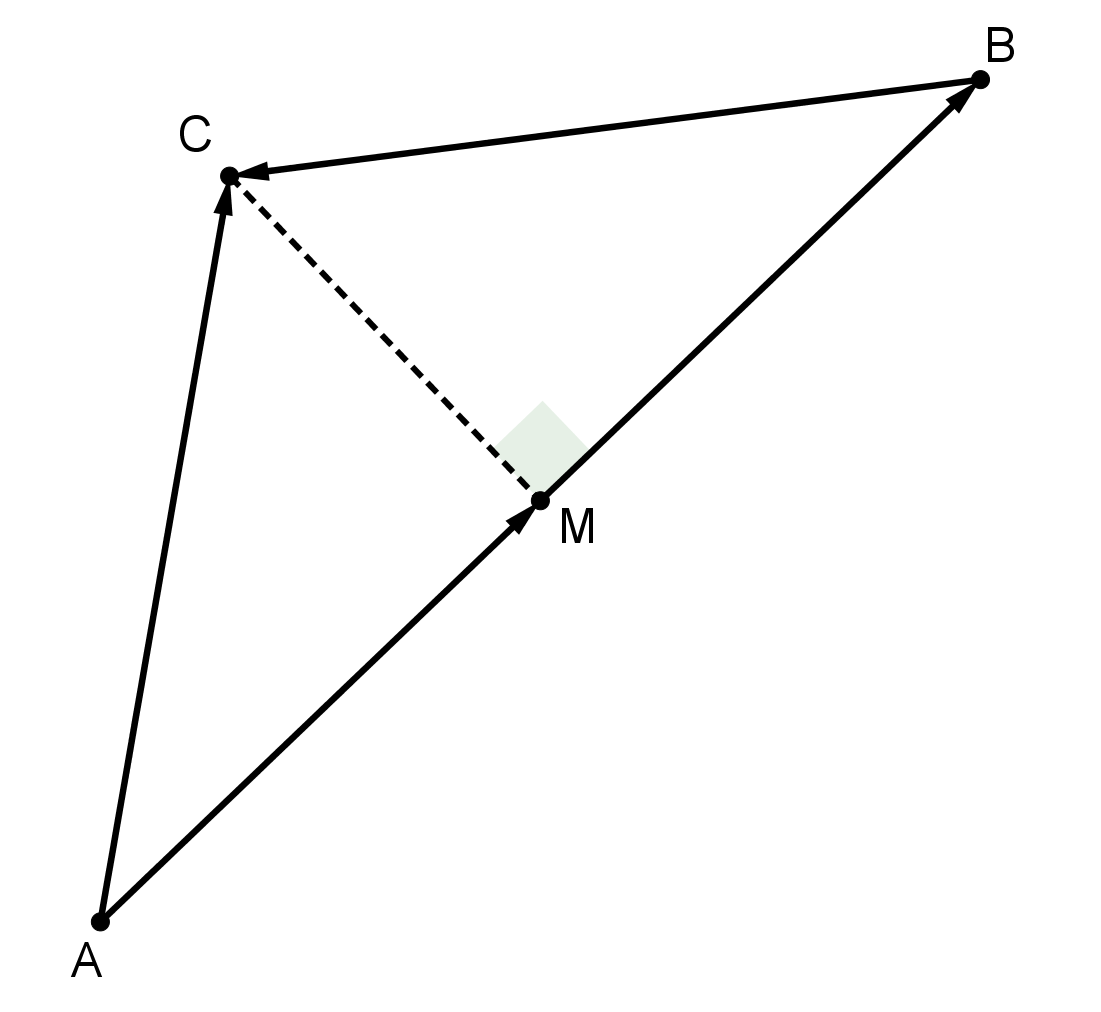
\includegraphics[width=0.5\textwidth]{1.png}
  \caption{ }
  \label{fig:1.2.7.1}
\end{figure}
\end{solution}
\begin{question}
  证明:若$u$是单位向量,则秩一矩阵$P=uu^T$是一个射影矩阵.它有性
  质(i)和(ii).选取$u=\frac{a}{||a||}$,$P$成为到$a$张成的直线上的射
  影,且$Pb$是点$p=\overline{x}a$:秩一的射影恰恰对应着一个未知量的最小二
  乘问题.
\end{question}
\begin{solution}
  我们知道,$u(u^Tu)^{-1}u^T$是到$u$张成的子空间上的射影矩阵.由于$u$是单
  位向量,因此$u^Tu=1$.因此$u(u^Tu)^{-1}u^T=uu^T$是到$u$张成的子空间上的
  射影矩阵.
\end{solution}
\begin{question}
  把$x-y$平面射影到$y$轴上的$2\times 2$矩阵是什么?
\end{question}
\begin{solution}
  $
  \begin{pmatrix}
    0\\
    1
  \end{pmatrix}
  \begin{pmatrix}
    0&1
  \end{pmatrix}=
  \begin{pmatrix}
    0&0\\
    0&1
  \end{pmatrix}.  $
\end{solution}
\begin{question}
  证明:对一组测量值$y_1,y_2,\cdots,y_m$,用一条水平直线(换句话说,用一
  个常值函数$y=C$)得到的最小二乘意义下的最佳拟合,是它们的平均值
$$
C=\frac{y_1+y_2+\cdots+y_m}{m}
$$
(与练习3.2.1比较)用统计术语来说,使$E^2=(y_1-y)^2+\cdots+(y_m-y)^2$极
小化的选择$\overline{y}$是样本的均值,而所得的$E^2$是均方差$\sigma^2$.
\end{question}
\begin{solution}
$$
\begin{pmatrix}
  1\\
1\\
\vdots\\
1
\end{pmatrix}
\begin{pmatrix}
  D
\end{pmatrix}=
\begin{pmatrix}
  y_1\\
y_2\\
\vdots\\
y_m
\end{pmatrix}.
$$
矩阵$A=
\begin{pmatrix}
  1\\
1\\
\vdots\\
1
\end{pmatrix},
$射影矩阵$P$是个$m\times m$矩阵,且
$$
\overline{D}=(A^TA)^{-1}A^Tb=\frac{1}{m}A^Tb=\frac{y_1+y_{2}+\cdots+y_{m}}{m}.
$$
\end{solution}
\begin{question}
  求下列测量值的最佳直线拟合,并简述解答:当$t=-1$时$y=2$,$t=0$时
  $y=0$,$t=1$时$y=-3$,$t=2$时$y=-5$.
\end{question}
\begin{solution}
  设拟合这些点的最佳直线是$y=Dx+C$.我们得到不相
  容的线性方程组:
$$
\begin{pmatrix}
  1&-1\\
  1&0\\
  1&1\\
  1&2
\end{pmatrix}
\begin{pmatrix}
  C\\
D
\end{pmatrix}=
\begin{pmatrix}
  2\\
0\\
-3\\
-5
\end{pmatrix}.
$$
令矩阵$A=
\begin{pmatrix}
  1&-1\\
  1&0\\
  1&1\\
  1&2
\end{pmatrix}
$,$b=
\begin{pmatrix}
  2\\
0\\
-3\\
-5
\end{pmatrix},
$
解得
$$
\begin{pmatrix}
  \overline{C}\\
\overline{D}
\end{pmatrix}=(A^TA)^{-1}A^Tb=
\begin{pmatrix}
  -\frac{3}{10}\\
-\frac{12}{5}
\end{pmatrix}.
$$
所以最佳拟合直线的方程是$y=-\frac{12}{5}x-\frac{3}{10}$.
\end{solution}
\begin{question}
  假如不用直线而改用抛物线$y=C+Dt+Et^2$来拟合上述练习中的数据,那么在
  由四组测量值得到的不相容方程组$Ax=b$中,系数矩阵$A$,未知向量$x$和数
  据向量$b$各是什么?不要求计算$\overline{x}$.
\end{question}
\begin{solution}
  $A=
  \begin{pmatrix}
    1&-1&1\\
    1&0&0\\
    1&1&1\\
    1&2&4
  \end{pmatrix},
$未知向量$x=
\begin{pmatrix}
  C\\
D\\
E
\end{pmatrix},
$数据向量$b=
\begin{pmatrix}
  2\\
0\\
-3\\
-5
\end{pmatrix}.
$
\end{solution}
\section{正交基,正交矩阵和Gram-Schmidt正交化}
\begin{question}
\begin{itemize}
\item 写出对下述数据的关于$y=C+Dt$拟合的四个方程
$$
y=-4,\mbox{当}t=-2;y=-3,\mbox{当}t=-1
$$
$$
y=-1,\mbox{当}t=1;y=0,\mbox{当}t=2
$$
证明这些列向量是正交的并化成单位向量.在新的问题$Ax=b$中未知数$c$和$d$
是什么?
\item 找出最佳直线.作图并写出误差$E^2$.
\item 用原来的两个未知数,四个方程组成的方程组来解释误差为零的事实,右
  边的$b$相应的列空间在什么地方?它的射影$P$是什么?
\end{itemize}
\end{question}
\begin{solution}
$$
  \begin{pmatrix}
 1&-2\\
 1&-1\\
 1&1\\
 1&2   
  \end{pmatrix}
  \begin{pmatrix}
    C\\
D
  \end{pmatrix}=
  \begin{pmatrix}
    -4\\
    -3\\
    -1\\
    0
  \end{pmatrix}.
$$
因为
$$
\begin{pmatrix}
  1&1&1&1
\end{pmatrix}
\begin{pmatrix}
  -2\\
-1\\
1\\
2
\end{pmatrix}=0,
$$
所以这些列向量是正交的.将这些向量化成单位向量,可得依次为
$$
\begin{pmatrix}
  \frac{1}{2}\\
\frac{1}{2}\\
\frac{1}{2}\\
\frac{1}{2}
\end{pmatrix},
\begin{pmatrix}
  \frac{-2}{\sqrt{10}}\\
\frac{-1}{\sqrt{10}}\\
\frac{1}{\sqrt{10}}\\
\frac{2}{\sqrt{10}}
\end{pmatrix}.
$$
新的问题是
$$
\begin{pmatrix}
  \frac{1}{2}&\frac{-2}{\sqrt{10}}\\
  \frac{1}{2}&\frac{-1}{\sqrt{10}}\\
  \frac{1}{2}&\frac{1}{\sqrt{10}}\\
  \frac{1}{2}&\frac{2}{\sqrt{10}}
\end{pmatrix}
\begin{pmatrix}
  c\\
d
\end{pmatrix}=
\begin{pmatrix}
  -4\\
-3\\
-1\\
0
\end{pmatrix},
$$
其中$c=2C,d=\sqrt{10}D$.下面我们来解这个新的最小二乘问题.易得
$$
\overline{c}=
\begin{pmatrix}
  \frac{1}{2}&\frac{1}{2}&\frac{1}{2}&\frac{1}{2}
\end{pmatrix}
\begin{pmatrix}
  -4\\
-3\\
-1\\
0
\end{pmatrix}=-4,
$$
$$
d=
\begin{pmatrix}
  \frac{-2}{\sqrt{10}}&\frac{-1}{\sqrt{10}}&\frac{1}{\sqrt{10}}&\frac{2}{\sqrt{10}}
\end{pmatrix}
\begin{pmatrix}
  -4\\
-3\\
-1\\
0
\end{pmatrix}=\sqrt{10}.
$$
所以$\overline{C}=-2,\overline{D}=1$.所以最佳直线是$y=x-2$.我们发现这
条直线恰好过四个点,因此误差$E^2=0$.事实上,向量$
\begin{pmatrix}
  -4\\\
-3\\
-1\\
0
\end{pmatrix}
$就在矩阵$
\begin{pmatrix}
  1&-2\\
1&-1\\
1&1\\
1&2
\end{pmatrix}
$的列空间中.它的射影$P$就是向量$
\begin{pmatrix}
  -4\\
-3\\
-1\\
0
\end{pmatrix}
$本身.
\end{solution}
\begin{question}
  把向量$b=(0,3,0)$投影到{\color{red}单位}正交向量
  $a_1=(\frac{2}{3},\frac{2}{3},\frac{-1}{3})$和
  $a_2=(-\frac{1}{3},\frac{2}{3},\frac{2}{3})$上去,并求出它在$a_1,a_2$
  所在平面上的射影.
\end{question}
\begin{solution}
  向量$b$在$a_1$上的投影:
$$
a_1^Ta_1b^T=
\begin{pmatrix}
  \frac{2}{3}\\
\frac{2}{3}\\
\frac{-1}{3}
\end{pmatrix}
\begin{pmatrix}
  \frac{2}{3}&\frac{2}{3}&\frac{-1}{3}
\end{pmatrix}
\begin{pmatrix}
  0\\
3\\
0
\end{pmatrix}=
\begin{pmatrix}
  \frac{4}{9}&\frac{4}{9}&\frac{-2}{9}\\
  \frac{4}{9}&\frac{4}{9}&\frac{-2}{9}\\
  \frac{-2}{9}&\frac{-2}{9}&\frac{1}{9}
\end{pmatrix}
\begin{pmatrix}
  0\\
3\\
0
\end{pmatrix}=
\begin{pmatrix}
  \frac{4}{3}\\
\frac{4}{3}\\
\frac{-2}{3}
\end{pmatrix}.
$$
向量$b$在$a_2$上的投影:
$$
a_2^Ta_2b^T=
\begin{pmatrix}
  \frac{-1}{3}\\
\frac{2}{3}\\
\frac{2}{3}
\end{pmatrix}
\begin{pmatrix}
  \frac{-1}{3}&\frac{2}{3}&\frac{2}{3}
\end{pmatrix}
\begin{pmatrix}
  0\\
3\\
0
\end{pmatrix}=
\begin{pmatrix}
  \frac{1}{9}&\frac{-2}{9}&\frac{-2}{9}\\
  \frac{-2}{9}&\frac{4}{9}&\frac{4}{9}\\
  \frac{-2}{9}&\frac{4}{9}&\frac{4}{9}
\end{pmatrix}
\begin{pmatrix}
  0\\
3\\
0
\end{pmatrix}=
\begin{pmatrix}
  -\frac{2}{3}\\
  \frac{4}{3}\\
  \frac{4}{3}
\end{pmatrix}.
$$
所以向量$b$在$a_1,a_2$所在平面上的射影是
$$
\begin{pmatrix}
  \frac{4}{3}\\
  \frac{4}{3}\\
  \frac{-2}{3}
\end{pmatrix}+
\begin{pmatrix}
  \frac{-2}{3}\\
  \frac{4}{3}\\
  \frac{4}{3}
\end{pmatrix}=
\begin{pmatrix}
  \frac{2}{3}\\
  \frac{8}{3}\\
  \frac{2}{3}
\end{pmatrix}.
$$
\end{solution}
\begin{question}
  求出$b=(0,3,0)$到$a_3=(\frac{2}{3},-\frac{1}{3},\frac{2}{3})$上的射
  影,把三个一维射影加起来并解释得到的结果.为什么
  $P=a_1a_1^T+a_2a_2^T+a_3a_3^{T}$是单位阵?
\end{question}
\begin{solution}
$a_3^Ta_3b^T=
\begin{pmatrix}
  \frac{4}{9}&\frac{-2}{9}&\frac{4}{9}\\
  \frac{-2}{9}&\frac{1}{9}&\frac{-2}{9}\\
  \frac{4}{9}&\frac{-2}{9}&\frac{4}{9}
\end{pmatrix}
\begin{pmatrix}
  0\\
3\\
0
\end{pmatrix}=
\begin{pmatrix}
  -\frac{2}{3}\\
  \frac{1}{3}\\
  -\frac{2}{3}
\end{pmatrix}.
$
三个一维射影加起来的结果是向量$b$.这是肯定的,因为向量$b$就在向量
$a_1,a_2,a_3$张成的线性空间内.事实上,由于$a_1,a_2,a_3$形成
$\mathbf{R}^3$中的标准正交基,所以任何三维向量都在$a_1,a_2,a_3$张成的空
间中.所以任意三维向量在射影矩阵$a_1a_1^T+a_2a_2^T+a_3a_3^T$的作用下必为本
身,因此$a_1a_1^T+a_2a_2^T+a_3a_3^T$必为单位矩阵.
\end{solution}
\begin{question}
  若$Q_1,Q_2$都是正交矩阵,从而都满足(36),证明$Q_1Q_2$也是正交矩阵.
\end{question}
\begin{solution}
  $$ 
(Q_1Q_2)^T(Q_1Q_2)=Q_2^TQ_1^TQ_1Q_2=Q_2^TQ_2=I.
 $$
所以$Q_1Q_2$也是正交矩阵.
\end{solution}
\begin{question}
  若$u$是一个单位向量,证明$Q=I-2uu^T$是一个正交矩阵(它就是所谓
  Householder变换).当$u=(1,1,1)/\sqrt{3}$,具体算出$Q$来.
\end{question}
\begin{solution}
$$ 
Q^TQ=(I-2uu^T)^T(I-2uu^T)=(I-2uu^T)(I-2uu^T)=I-4uu^T+4(uu^T)(uu^T)=I-4uu^T+4u(u^Tu)u^T=I-4uu^T+4uu^T=I.
$$
所以$Q=I-2uu^T$是正交矩阵.事实上,此题的几何意义可参见题3.2.7.当
$u=(1,1,1)/\sqrt{3}$时,
$$
Q=
\begin{pmatrix}
  1&0&0\\
  0&1&0\\
  0&0&1
\end{pmatrix}-2
\begin{pmatrix}
  \frac{1}{\sqrt{3}}\\
  \frac{1}{\sqrt{3}}\\
  \frac{1}{\sqrt{3}}
\end{pmatrix}
\begin{pmatrix}
  \frac{1}{\sqrt{3}}&\frac{1}{\sqrt{3}}&\frac{1}{\sqrt{3}}
\end{pmatrix}=
\begin{pmatrix}
  \frac{1}{3}&-\frac{2}{3}&-\frac{2}{3}\\
  -\frac{2}{3}&\frac{1}{3}&-\frac{2}{3}\\
  -\frac{2}{3}&-\frac{2}{3}&\frac{1}{3}
\end{pmatrix}.
$$
\end{solution}
\begin{question}
  求一个位于第三列的向量,使得矩阵
$$
Q=
\begin{pmatrix}
  \frac{1}{\sqrt{3}}&\frac{1}{\sqrt{2}}& \\
  \frac{1}{\sqrt{3}}&0&\\
  \frac{1}{\sqrt{3}}&-\frac{1}{\sqrt{2}}&
\end{pmatrix}
$$
成为正交矩阵.这个向量必是一个单位向量而且与其它两个列向量正交.这个列向
量的选取有多大的自由度?验证$Q$的行向量同时自动成为标准正交的.
\end{question}
\begin{solution}
  该列向量的选取有两个自由度.该列向量可以是
$
\begin{pmatrix}
  \frac{1}{\sqrt{6}}\\
-\frac{2}{\sqrt{6}}\\
\frac{1}{\sqrt{6}}
\end{pmatrix},
$
也可以是$
\begin{pmatrix}
  -\frac{1}{\sqrt{6}}\\
  \frac{2}{\sqrt{6}}\\
  \frac{1}{\sqrt{6}}
\end{pmatrix}
$.
\end{solution}
\begin{question}
通过直接计算$v^Tv$来验证:对于标准正交向量组的任何组合
$v=x_1q_1+x_2q_2+\cdots+x_nq_n$,勾股定理均成立:
$$
||v||^2=x_1^2+\cdots+x_n^2
$$
用矩阵的形式来写,就是$v=Qx$,因此这就给出长度保持不变:$||Qx||^2=||x||^2$这
个事实的一个新的且更清楚的证明.  
\end{question}
\begin{solution}
  题目本身几乎就是解答.因此解答略.
\end{solution}
\begin{question}
  下列矩阵是正交的吗?
$$
Q=
\begin{pmatrix}
  \frac{1}{2}&\frac{1}{2}&\frac{1}{2}&\frac{1}{2}\\
  \frac{1}{2}&\frac{1}{2}&-\frac{1}{2}&-\frac{1}{2}\\
  \frac{1}{2}&-\frac{1}{2}&-\frac{1}{2}&\frac{1}{2}\\
  \frac{1}{2}&-\frac{1}{2}&\frac{1}{2}&-\frac{1}{2}
\end{pmatrix}.
$$
\end{question}
\begin{solution}
  是.
\end{solution}
\begin{question}
  应用Gram-Schmidt正交化过程于
$$
a_1=
\begin{pmatrix}
  0\\
0\\
1
\end{pmatrix},a_2=
\begin{pmatrix}
  0\\
1\\
1
\end{pmatrix},a_3=
\begin{pmatrix}
  1\\
1\\
1\\
\end{pmatrix}.
$$
并把结果写成$A=QR$的形式.
\end{question}
\begin{solution}
令$v_1=a_1$.
$$
v_2=a_2-\frac{a_2^Ta_1}{a_1^Ta_1}a_1=
\begin{pmatrix}
  0\\
1\\
1\\
\end{pmatrix}-\frac{1}{1}
\begin{pmatrix}
  0\\
0\\
1
\end{pmatrix}=
\begin{pmatrix}
  0\\
1\\
0
\end{pmatrix}.
$$
$$
v_3=a_3-\frac{a_3^Tv_1}{v_1^Tv_1}v_1-\frac{a_3^Tv_2}{v_2^Tv_2}v_2=
\begin{pmatrix}
  1\\
1\\
1\\
\end{pmatrix}-\frac{1}{1}
\begin{pmatrix}
  0\\
0\\
1
\end{pmatrix}-\frac{1}{1}
\begin{pmatrix}
  0\\
1\\
0
\end{pmatrix}=
\begin{pmatrix}
  1\\
0\\
0
\end{pmatrix}.
$$
且$q_1=\frac{v_1}{1}=v_1,q_2=\frac{v_2}{1}=v_2,q_3=\frac{v_3}{1}=v_3$.结果,
$$
a_1=q_1,a_2=q_2+q_1,a_3=q_3+q_2+q_1,
$$
因此
$$
\begin{pmatrix}
  a_1&a_2&a_3
\end{pmatrix}=
\begin{pmatrix}
  q_1&q_2&q_3
\end{pmatrix}
\begin{pmatrix}
  1&1&1\\
  0&1&1\\
  0&0&1
\end{pmatrix}.
$$即
$$
\begin{pmatrix}
  0&0&1\\
  0&1&1\\
  1&1&1
\end{pmatrix}=
\begin{pmatrix}
0&0 &1\\
0&1 &0\\
1&0 &0\\
\end{pmatrix}
\begin{pmatrix}
  1&1&1\\
  0&1&1\\
  0&0&1
\end{pmatrix}.
$$      
\end{solution}
\begin{question}
  把$A=
  \begin{pmatrix}
    3&0\\
    4&5
  \end{pmatrix}
$分解成QR.
\end{question}
\begin{solution}
  令$a_1=
  \begin{pmatrix}
    3\\
4
  \end{pmatrix}
$,$a_2=
\begin{pmatrix}
  0\\
5
\end{pmatrix}
$,且令$v_1=a_1=
\begin{pmatrix}
  3\\
4
\end{pmatrix}
$,
$$
v_2=a_2-\frac{a_2^Ta_1}{a_1^Ta_1}a_1=
\begin{pmatrix}
  0\\
5
\end{pmatrix}-\frac{20}{25}
\begin{pmatrix}
  3\\
4
\end{pmatrix}=
\begin{pmatrix}
  -\cfrac{12}{5}\\
  \cfrac{9}{5}
\end{pmatrix}.
$$
令$q_1=\frac{v_1}{||v_1||}=
\begin{pmatrix}
  \cfrac{3}{5}\\
  \cfrac{4}{5}
\end{pmatrix}
$,$q_2=\frac{v_2}{||v_2||}=
\begin{pmatrix}
  -\cfrac{4}{5}\\
  \cfrac{3}{5}
\end{pmatrix}
$.因此
$$
a_1=v_1=||v_1||q_1=5q_1,a_2=v_2+\frac{4}{5}v_1=||v_2||q_2+\frac{4}{5}||v_1||q_1=3q_2+4q_1.
$$
即
$$
\begin{pmatrix}
  a_1&a_2
\end{pmatrix}=
\begin{pmatrix}
  q_1&q_2
\end{pmatrix}
\begin{pmatrix}
  5&4\\
0&3
\end{pmatrix}.
$$
即
$$
\begin{pmatrix}
  3&0\\
  4&5
\end{pmatrix}=
\begin{pmatrix}
  \frac{3}{5}&-\frac{4}{5}\\
  \frac{4}{5}&\frac{3}{5}
\end{pmatrix}
\begin{pmatrix}
  5&4\\
  0&3
\end{pmatrix}.
$$
\end{solution}
\begin{question}
  把
$$
a_1=
\begin{pmatrix}
  1\\
2\\
2
\end{pmatrix},a_2=
\begin{pmatrix}
  1\\
3\\
1
\end{pmatrix}
$$
的Gram-Schimidt正交化过程表为A=QR的形式.给定$n$个具有$m$个分量的向量
$a_i$,A,Q和R的形状各是什么样?
\end{question}
\begin{solution}
  令$v_1=a_1=
  \begin{pmatrix}
    1\\
2\\
2
  \end{pmatrix}
$,$v_2=a_2-\frac{a_2^Tv_1}{v_1^Tv_1}v_1=
\begin{pmatrix}
  1\\
3\\
1
\end{pmatrix}-\frac{9}{9}
\begin{pmatrix}
  1\\
2\\
2\\
\end{pmatrix}=
\begin{pmatrix}
  0\\
1\\
-1
\end{pmatrix}.
$
令
$$ 
q_1=\frac{v_1}{||v_1||}=
\begin{pmatrix}
  \frac{1}{3}\\
\frac{2}{3}\\
\frac{2}{3}
\end{pmatrix},q_2=\frac{v_2}{||v_2||}=
\begin{pmatrix}
0\\
\frac{1}{\sqrt{2}}\\
-\frac{1}{\sqrt{2}}
\end{pmatrix}.
 $$
因此,
$$
a_1=v_1=||v_1||q_1=3q_1,a_2=v_1+v_2=||v_1||q_1+||v_2||q_2=3q_1+\sqrt{2}q_2,
$$
即
$$
\begin{pmatrix}
  a_1&a_2
\end{pmatrix}=
\begin{pmatrix}
  q_1&q_2
\end{pmatrix}
\begin{pmatrix}
  3&3\\
0&\sqrt{2}
\end{pmatrix}.
$$
因此
$$
\begin{pmatrix}
  1&1\\
  2&3\\
  2&1
\end{pmatrix}=
\begin{pmatrix}
  \frac{1}{3}&0\\
  \frac{2}{3}&\frac{1}{\sqrt{2}}\\
  \frac{2}{3}&\frac{-1}{\sqrt{2}}
\end{pmatrix}
\begin{pmatrix}
  3&3\\
  0&\sqrt{2}
\end{pmatrix}.
$$
给定$n$个具有$m$个分量的向量$a_i$,$A$是$m\times n$矩阵,$Q$是$m\times
n$矩阵,$R$是$n\times n$矩阵.
\end{solution}
\begin{question}
  对上题的$A$及$b=(1,1,1)^T$,使用$A=QR$来解最小二乘问题$Ax=b$.
\end{question}
\begin{solution}
  $$ 
\overline{x}=R^{-1}Q^Tb=
\begin{pmatrix}
  \frac{1}{3}&\frac{-1}{\sqrt{2}}\\
  0&\frac{1}{\sqrt{2}}
\end{pmatrix}
\begin{pmatrix}
  \frac{1}{3}&\frac{2}{3}&\frac{2}{3}\\
  0&\frac{1}{\sqrt{2}}&\frac{-1}{\sqrt{2}}
\end{pmatrix}
\begin{pmatrix}
  1\\
1\\
1
\end{pmatrix}=
\begin{pmatrix}
  \frac{1}{3}\\
0
\end{pmatrix}.
$$  
\end{solution}
\begin{question}
 若$A=QR$,求出$A$的列向量空间的射影矩阵$P$的简单公式.
\end{question}
\begin{solution}
\begin{align*}
P&=A(A^TA)^{-1}A^T
\\&=QR[(QR)^TQR]^{-1}(QR)^T
\\&=QR(R^TQ^TQR)^{-1}R^TQ^T
\\&=QR(R^TR)^{-1}R^TQ^T
\\&=QRR^{-1}(R^T)^{-1}R^TQ^T
\\&=QQ^T.
\end{align*}
\end{solution}
\begin{question}
  证明下述两个步骤
$$
w=c-\frac{v_1^Tc}{v_1^Tv_1}v_1,v_3=w-\frac{v_2^Tw}{v_2^Tv_2}v_2
$$
得出与公式(40)相同的第三个方向$v_3$.这是一个修改了的Gram-Schimidt正交
化过程的例子.在这个过程中为保证数值稳定,一次只减去一个射影.
\end{question}
\begin{solution}
  $$ 
v_3=w-\frac{v_2^Tw}{v_2^Tv_2}v_2=\left(c-\frac{v_1^Tc}{v_1^Tv_1}v_1\right)-\frac{v_2^T\left(c-\frac{v_1^Tc}{v_1^Tv_1}v_1\right)}{v_2^Tv_2}v_2=c-\frac{v_1^Tc}{v_1^Tv_1}v_1-\frac{v_2^Tc}{v_2^Tv_2}v_2.
 $$
\end{solution}
\begin{question}
  求向量
  $v=(\frac{1}{\sqrt{2}},\frac{1}{\sqrt{4}},\frac{1}{\sqrt{8}},\cdots)$
  的长度以及函数$f(x)=e^x$(在区间$0\leq x\leq 1$上)的长度.在这个区间内
  $e^x$与$e^{-x}$的内积是什么?
\end{question}
\begin{solution}
  $$ 
||v||=\sqrt{\frac{1}{2}+\frac{1}{4}+\frac{1}{8}+\cdots}=1.
 $$
$f(x)=e^x$在$[0,1]$上的长度为
$$
\int_0^1(e^x)^2dx=\frac{1}{2}e^2-\frac{1}{2}.
$$
在区间$[0,1]$上$e^x$与$e^{-x}$的内积是
$$
\int_0^1e^xe^{-x}dx=1.
$$
\end{solution}
\begin{question}
  用令导数为$0$的方法求$b_1$的值使得下式极小化:
$$
||b_1\sin x-y||^2=\int_0^{2\pi}(b_1\sin x-y(x))^2dx
$$
请与Fourier系数(47)做一比较.若$y(x)=\cos x$,$b_1$等于什么?
\end{question}
\begin{solution}
令$E(x)^2=||b_1\sin
x-y||^2=\int_0^{2\pi}[b_1^2\sin^2x+y(x)^2-2b_1y(x)\sin x]dx$.则令
$$
\frac{\partial E(x)^2}{\partial b_1}=2b_1\int_0^{2\pi}\sin^2x
dx-2\int_0^{2\pi}y(x)\sin xdx=0,
$$
解得
$$
b_1=\frac{\int_0^{2\pi}y(x)\sin xdx}{\int_0^{2\pi}\sin^2xdx}.
$$
若$y(x)=\cos x$,$b_1=0$.
\end{solution}
\begin{question}
  求分段函数$y(x)$的Fourier系数$a_0,a_1$和$b_1$,$y(x)$在区间$0\leq
  x\leq \pi$上等于$1$而在区间$\pi<x\leq 2\pi$上等于$0$:
$$
a_0=\frac{y^T1}{1^T1},a_1=\frac{y^T\cos x}{(\cos x)^T(\cos
  x)},b_1=\frac{y^T\sin x}{(\sin x)^T\sin x}.
$$
\end{question}
\begin{solution}
  $$ 
a_0=\frac{y^T1}{1^T1}=\frac{\int_0^{2\pi}y(x)dx}{\int_0^{2\pi}1dx}=\frac{\pi}{2\pi}=\frac{1}{2}.
 $$
$$
a_1=\frac{y^T\cos x}{(\cos x)^T(\cos x)}=\frac{\int_0^{2\pi}y(x)\cos xdx}{\int_0^{2\pi}\cos^2xdx}=0,
$$
$$
b_1=\frac{y^T\sin x}{(\sin x)^T\sin x}=\frac{\int_0^{2\pi}y(x)\sin xdx}{\int_0^{2\pi}\sin^2xdx}=\frac{2}{\pi}.
$$
\end{solution}
\begin{question}
  求下一个Legendre多项式——一个与$1$,$x$和$x^2-\frac{1}{3}$正交的多项式.
\end{question}
\begin{solution}
$$
x^3-\frac{(x^3)^T1}{1^T1}1-\frac{(x^3)^Tx}{x^Tx}x-\frac{(x^3)^T(x^2-\frac{1}{3})}{(x^2-\frac{1}{3})^T(x^2-\frac{1}{3})}(x^2-\frac{1}{3})=x^3-\frac{3}{5}x.
$$
\end{solution}
\begin{question}
 对区间$-1\leq x\leq 1$上的抛物线$y=x^2$来说,与它最接近的直线是什么?
\end{question}
\begin{solution}
 首先,$1$与$x$在$[-1,1]$上是正交的.由Gram-Schmidt正交化过程,可得欲求直
 线为
$$
\frac{(x^2)^T1}{1^T1}1+\frac{(x^2)^Tx}{x^Tx}x=\frac{1}{3}.
$$
所以直线为$y=\frac{1}{3}$.
\end{solution}
\end{document}